\chapter{Experimental evaluation}
\label{chap:evaluation}

Now we evaluate the proposed configurations from the chapter \ref{chap:framework_configuration} that we implemented in the chapter \ref{chap:protype_software_application}. First, we describe the data that we used for evaluation. Then, we evaluate our RAG approaches, the generated suggestions of domain elements, and the generated descriptions. Finally, we present results of our user-based evaluation of our prototype application.


\section{Evaluation domains}

To assess the quality of our generators, we used six domains with their domain description and manually created reference domain models. These domains can be found in our data repository\footnote{\url{https://github.com/dataspecer/domain-modeling-benchmark}}. Table \ref{tab:reference-model-size} summarizes the size of these reference models.

\begin{table}[!h]
    \scriptsize
    \centering
    \setlength{\tabcolsep}{0.5em}
    \begin{tabular}{lcccccc}
         & Aircrafts & Papers & Farming & Zoos & Colleges & Vehicles \\
    \toprule
    \addlinespace
         \# classes      & 8  & 7  & 14 & 14 & 63 & 66 \\
         \# attributes   & 10 & 12 & 15 & 26 & 14 & 72 \\
         \# associations & 8  & 9  & 9  & 24 & 67 & 46 \\
    \addlinespace
    \bottomrule
    \addlinespace
    \end{tabular}
    \caption{The size of the reference domain models}
    \label{tab:reference-model-size}
\end{table}


We categorize the domains into two groups.
The first group contains three domains: \emph{aircraft manufacturing}, \emph{conference papers}, and \emph{farming}.
They are characterized by simpler descriptions with a limited scope of concepts.
For each domain, we manually created three semantically equivalent domain descriptions in three different styles.
\emph{Analytical} descriptions are written with analytical precision, describing each concept rigorously, unambiguously, and preferably with a consistent sequence of sentences.
\emph{Eclectic} are written as a collection of less structured knowledge from different stakeholders, each describing the domain from a different point of view.
\emph{Educational} emphasize the most important concepts at the beginning, where only essential aspects are described, followed by adding more details about the concepts later in the description.


\subsubsection{Annotated domain descriptions}

To assess the quality of our RAG approaches, for each domain description we also manually created corresponding annotated domain description. Each annotated domain description contains tags that for each domain element from the corresponding reference domain model determine the parts that contain information about this domain element. Here is an example of the original domain description and the corresponding annotated domain description from the \emph{farming} domain: \\

\noindent{}Domain description: \textit{A farmer is an individual engaged in agriculture, growing and harvesting crops, and is identified uniquely by a name that is used to refer to the farmer from various documentation, statistical reporting, etc.} \\

\noindent{}Annotated domain description: \textit{\textbf{<farmer>}A farmer is an individual engaged in agriculture, growing and harvesting crops\textbf{</farmer>}, and \textbf{<name>}is identified uniquely by a name that is used to refer to the farmer from various documentation, statistical reporting, etc.\textbf{</name>}}

The corresponding reference model contains the class \textit{farmer} with the attribute \textit{name}. In the annotated text the parts between the opening tag ``\textbf{<farmer>}'' and the closing tag ``\textbf{</farmer>}'' capture the information about the class \textit{farmer}. Similarly, the opening tag ``\textbf{<name>}'' and the closing tag ``\textbf{</name>}'' captures the information about the attribute \textit{name} of the class \textit{farmer}.

The annotated domain description can contain multiple tags with the same name. After an opening tag can follow another opening tag if it has a different name but each tag must be first opened and then closed.


\section{RAG evaluation}
\label{sec:filtering_evaluation}

\subsection{Evaluation methodology}

As already mentioned, for the RAG evaluation we use the annotated domain descriptions.

\subsubsection{Recall}

For a domain element $e$ let $Y_e$ be the set of expected relevant parts that are marked by the tags with the name equal to the $name(e)$. Let $X_e \subseteq Y_e$ be the set of parts from $Y_e$ that the selected RAG approach marked as relevant based on the $name(e)$ if $e$ is a class, otherwise based on the $name(source(e))$. Now when given a domain description with its reference domain model containing a set of domain elements denoted by $E$ where the $E$ can be a set of classes, attributes, or associations. The recall $R$ is computed as:

\[ R = \dfrac{\sum_{e \in E}|Y_e|}{\sum_{e \in E}|X_e|}. \]

\noindent{}where $|Y_e|$ denotes the size of the set $Y_e$ and $|X_e|$ denotes the size of the set $X_e$.


\subsubsection{Precision}

For a class $c$ and domain description $T$ let $Y_{c}$ be the set of expected relevant parts from the annotated domain descriptions of the class $c$ and of the attributes and associations with the name of their source class equal to the $name(c)$. Now let $Z_{c}$ be the set of chunks from the given domain description that the selected RAG approach marked as relevant based on the class $c$. Then the precision $P_{c}$ for the class $c$ and the domain description $T$ is computed as:

\[ P = \dfrac{\sum_{c \in C}|Y_c|}{\sum_{c \in C}|Z_c|}. \]

We do not compute the precision separately for classes, attributes, and associations as the goal of our RAG approach is to find relevant information for a given source class but not to find the information about classes, attributes, and associations separately.


\subsection{Selected models}

For our semantic approach, we use the \textit{SentenceTransformers}\footnote{\url{https://sbert.net/}} library with the model \textit{all-MiniLM-L6-v2}\footnote{\url{https://huggingface.co/sentence-transformers/all-MiniLM-L6-v2}}. It is a symmetric embedding model intended for encoding sentences and short paragraphs. As a comparison function, we use \textit{cosine-similarity}.

Our syntactic approach uses the \textit{MorphoDiTa} tool \cite{Strakova2014} with the \textit{english-morphium-wsj-140407} model for converting English words into lemmas \cite{Straka2014}.


\subsection{Results}

In the section \ref{sec:rag_configurations}, we introduced our semantic and syntactic RAG approach. For comparing these approaches now we also introduce the no-filtering approach where the domain description is not filtered at all. The table \ref{tab:filtering-results} contains the measured results:

\begin{table}[!h]
    \scriptsize
    \centering
    \setlength{\tabcolsep}{0.5em}
    \begin{tabular}{lcccc}

    \toprule
         & Recall classes & Recall attributes & Recall associations & Precision \\
    \toprule
    
    \addlinespace
         no-filtering      & 1.00  & 1.00  & 1.00 & 0.06 \\
    	 syntactic-baseline & 0.87 & 0.79 & 0.84 & 0.55 \\
         syntactic-pronouns-naive & 0.93  & 0.91  & 0.90 & 0.49 \\
         semantic-baseline & 0.99 & 0.96 & 0.97 & 0.10 \\
         semantic-pronouns-naive & 1.00 & 0.98 & 0.98 & 0.10 \\
    \addlinespace
    \bottomrule
    \addlinespace
    \end{tabular}
    \caption{The size of the reference domain models}
    \label{tab:filtering-results}
\end{table}

As expected, the no-filtering approach gets the highest possible recall but also gets the lowest precision.

In the syntactic approach, the naive pronouns detection improves the recall significantly but slightly decreases the precision as chunks starting with a pronoun also contain the previous chunk. This approach can probably offer the best performance as it has the highest precision of all the measured approaches. To improve its recall, the domain description can be manually pre-processed to remove some problematic constructs such as unexpressed subjects.

The semantic approach almost matches the recall of the no-filtering approach but it has a higher precision. The naive pronouns approach slightly increases the recall while maintaining the same precision.

Overall, when recall is the most important then the no-filtering approach or the semantic approach can be used. On the other hand, when precision is the most important and we do not care about losing some domain element suggestions then the syntactic approach is the most suitable.


\section{Selected LLMs}

Running a LLM requires a lot of resources, therefore frequently using a LLM through some API can cost a lot of money. Thus, we run open-source LLMs locally with LLaMA.cpp server\footnote{\url{https://github.com/ggerganov/llama.cpp/blob/master/examples/server/README.md}}. Our hardware is limited to a single NVIDIA A100 40GB GPU.

\subsection{Limitations}

Because of our hardware limitation we use Mixtral-8x7B\footnote{\url{https://huggingface.co/TheBloke/Mixtral-8x7B-Instruct-v0.1-GGUF/blob/main/mixtral-8x7b-instruct-v0.1.Q5_K_M.gguf}} (medium-sized LLM) \cite{Jiang2024} and Llama-3-70B\footnote{\url{https://huggingface.co/bartowski/Meta-Llama-3-70B-Instruct-GGUF/blob/main/Meta-Llama-3-70B-Instruct-Q5_K_M.gguf}} (relatively large-size LLM) both in quantized variation where on average they have 5 bits per parameter.


\subsection{Mixtral-8x7B}

Mixtral-8x7B has the context window size of 32k tokens and it outperforms or matches ChatGPT-3.5 across many benchmarks \cite{Jiang2024}. This LLM has in total 47B parameters, which are distributed among 8 experts. To achieve faster output generation, for each generated token 2 of the 8 experts are selected. The selection of the experts can be different for each token \cite{Jiang2024}.


\subsection{Llama-3-70B}

Llama-3-70B has an 8k tokens context window size and as of writing this thesis, it is the state-of-the-art LLM at the 70B parameters scale\footnote{\url{https://ai.meta.com/blog/meta-llama-3/}}.


%\section{Limitations}
%
%\begin{itemize}
%\item we used one domain modeling expert for evaluating attributes and associations, we used one student for evaluating classes, and domain elements descriptions
%\item we did preliminary experiments on most of the configurations with one middle sized domain description and then used more domain descriptions for the most promising configurations
%\end{itemize}


\section{Evaluation of generated domain elements}

First, we describe the rules for evaluating the domain elements then we present a preliminary evaluation where we evaluate generated attributes and associations with many different configurations of prompting techniques, RAG approaches, and LLMs with the domain description \textit{zoological gardens-00}\footnote{\url{https://github.com/dataspecer/domain-modeling-benchmark/blob/main/manual\%20evaluation\%20domains/zoological\%20gardens/domain-description-00.txt}}. Then, we select the most promising configurations and evaluate them on all our other domain descriptions.


\subsection{Manual assessment of generated suggestions}

Each generated suggestion was manually assessed by a human evaluator who recorded the assessment in the evaluation tables in columns \emph{Matches class}, \emph{Matches attribute}, and \emph{Matches association}.
\emph{Semantic correspondence} between a suggested $X'$ and a reference $X$ $\in$ $M$ is essential for the evaluation.
%The evaluator decides based on the metadata provided about $X'$ and $X$.
If the question \emph{Can we model $X$ also as $X'$?} can be answered positively, $X'$ \emph{semantically corresponds to} $X$.

\begin{table}[!h]
    \scriptsize
    \centering
    \setlength{\tabcolsep}{0.5em}
    \begin{tabular}{lccc}
                     & \emph{Matches class}        & \emph{Matches attribute} & \emph{Matches association} \\
\toprule
\addlinespace
        $gen_c(T)$   & $name(X)$ $\vert$ * $\vert$ & \emph{N/A}  & \emph{N/A} \\
                     & $name(X_1)$;$\ldots$        & \emph{N/A}  & \emph{N/A} \\
\addlinespace
\midrule
\addlinespace
        $gen_a(T,C)$ & $name(D)$ $\vert$ *         & $name(X)$ $\vert$ * $\vert$ & $name(X)$ $\vert$ * $\vert$ \\
        $gen_{r1}(T,C)$ &                             & :$name(X)$ $\vert$ :* $\vert$ & :$name(X)$ $\vert$ :* $\vert$ \\
                     &                             & $name(X_1)$;$\ldots$        & $name(X_1)$;$\ldots$ \\
\addlinespace
\bottomrule
    \end{tabular}
    \caption{Summary of manual evaluation rules}
    \label{tab:manual-assessment-of-suggestions}
\end{table}

To limit subjectivity, we requested that the manual evaluation is carried out according to the rules summarized in Table \ref{tab:manual-assessment-of-suggestions}.
If the class $X'$ suggested by $gen_c(T)$ corresponds to a single class $X$, we record $name(X)$ in \emph{Matches class}.
%The correspondence is determined by whether $name(X')$ refers to the same conceptual entity as $name(X)$.
The assessment considers both the occurrences of $name(X')$ within $T$ and how $X$ is structured within $M$.
If $X'$ does not correspond to any class in $M$, but the evaluator considers it valid from the semantic point of view based on $T$, we record an asterisk (*) in \emph{Matches class}.
%This indicates that according to the judgment of the evaluator, $X'$ represents a concept that could be modeled in $M$ based on its relevance and presence in $T$.
This scenario can arise especially in more complex domains where not all concepts in the domain description are modeled, or a concept can be modeled with an attribute instead of an association and a class.
If $X'$ does not correspond to any single class in $M'$, but its $name(X')$ corresponds to a list of classes $X_1$, $\ldots$, $X_n$ $\in$ $M$, their names are concatenated to $name(X_1)$;$\ldots$;$name(X_n)$ which we record in \emph{Matches classes}.
This corresponds to scenarios where domain models are more coarse-grained.

For a property $X'$ suggested by $gen_a(T,C)$ and $gen_r(T,C)$, we consider similar rules with some differences.
If $X'$ is a suggested attribute, it can also correspond to an association $X$ and vice versa.
This scenario arises in practice, where properties can be modeled as attributes or associations interchangably based on the desired level of semantic and structural detail of the resulting domain model.
Therefore, $name(X)$ is recorded in \emph{Matches attribute} if $X$ is a reference attribute or \emph{Matches association} if $X$ is a reference association.
Moreover, $X'$ must correspond to $X$ also in its source class and, if $X'$ is an association, in its target classes.
$X'$ can be suggested in the reverse direction of $X$.
The asterisk (*) and the lists are used in the same way as for the classes.
In addition, when $X'$ corresponds to an association $X$ then $name(D)$ of the class at the other end of $X$ than the end with $C$ is recorded in \emph{Matches class}.
This corresponds to a scenario where a domain modeler models $D$ not in the step of identifying classes in $T$, but when modeling $X$ starting in $C$.
%In this step, the designer creates $D$ which we record by $name(D)$ in \emph{Matches class}.
When $X'$ corresponds to an association that is not in $M$, the class at the other end of this association is a class $D$ in $M$, which we record again with $name(D)$ in \emph{Matches class}.
Last but not least, it might happen that $X'$ corresponds to $X$ only when the correspondence requirement in the source/target class is relaxed so that the classes at the ends of $X'$ can be subclasses or superclasses of the corresponding classes at the ends of $X$.
In that case, we write a colon(:) followed by $name(X)$ to \emph{Matches attribute} or \emph{Matches class}.
We write a colon followed by an asterisk (:*) if $X'$ makes sense, but should be modeled for a subclass or superclass of $C$. \\

\noindent{}TODO: Provide examples for the more complicated rules


\subsection{Preliminary evaluation results for attributes and associations}
\label{sec:preliminary_attributes_associations}

The table \ref{tab:preliminary-mixtral} shows preliminary results for generating attributes and associations with \emph{Mixtral-8x7B} and the table \ref{tab:preliminary-llama} shows preliminary results for generating attributes and associations with \emph{Llama-3-70B}.

\begin{table}[!h]
    \scriptsize
    \centering
    \setlength{\tabcolsep}{0.5em}
    \begin{tabular}{lcccccc}
    \toprule
         & & Attributes & & & Associations & \\
     \toprule
         & Recall & Precision & $F_1$ & Recall & Precision & $F_1$ \\
    \toprule
    
    \addlinespace
         baseline-none        & 0.73 & 0.33 & 0.45 & 0.54 & 0.22 & 0.31 \\
    	 baseline-semantic    & 0.73 & 0.35 & 0.47 & 0.75 & 0.27 & 0.40 \\
         baseline-syntactic   & 0.73 & 0.38 & 0.50 & 0.62 & 0.38 & 0.47 \\
         CoT-none             & 0.62 & 0.34 & 0.44 & 0.75 & 0.50 & 0.60 \\
         CoT-semantic         & 0.58 & 0.58 & \textbf{0.58} & 0.67 & 0.39 & 0.49 \\
         CoT-syntactic        & 0.88 & 0.43 & \textbf{0.58} & 0.71 & 0.53 & 0.61 \\
         N-shot-none          & 0.85 & 0.23 & 0.36 & 0.71 & 0.35 & 0.47 \\
         N-shot-semantic      & 0.85 & 0.32 & 0.46 & 0.83 & 0.47 & 0.60 \\
         N-shot-syntactic     & 0.88 & 0.38 & 0.53 & 0.83 & 0.59 & \textbf{0.69} \\
         CoT+N-shot-none      & 0.92 & 0.28 & 0.43 & 0.46 & 0.40 & 0.43 \\
         CoT+N-shot-semantic  & 0.88 & 0.35 & 0.50 & 0.79 & 0.49 & 0.60 \\
         CoT+N-shot-syntactic & 0.92 & 0.37 & 0.53 & 0.79 & 0.53 & 0.63 \\
    \addlinespace
    \bottomrule
    \addlinespace
    \end{tabular}
    \caption{Preliminary evaluation with Mixtral-8x7B strict variation only}
    \label{tab:preliminary-mixtral}
\end{table}


\begin{table}[!h]
    \scriptsize
    \centering
    \setlength{\tabcolsep}{0.5em}
    \begin{tabular}{lcccccc}
    \toprule
         & & Attributes & & & Associations & \\
     \toprule
         & Recall & Precision & $F_1$ & Recall & Precision & $F_1$ \\
    \toprule
    
    \addlinespace
         baseline-none        & 0.96 & 0.80 & \textbf{0.87} & 0.71 & 0.34 & 0.46 \\
    	 baseline-semantic    & 0.88 & 0.64 & 0.74 & 0.79 & 0.49 & 0.60 \\
         baseline-syntactic   & 0.92 & 0.59 & 0.72 & 0.89 & 0.59 & 0.69 \\
         CoT-none             & 0.88 & 0.72 & 0.79 & 0.67 & 0.59 & 0.63 \\
         CoT-semantic         & 0.85 & 0.70 & 0.77 & 0.88 & 0.56 & 0.68 \\
         CoT-syntactic        & 0.92 & 0.52 & 0.66 & 0.88 & 0.54 & 0.67 \\
         N-shot-none          & 0.92 & 0.66 & 0.77 & 0.79 & 0.60 & 0.68 \\
         N-shot-semantic      & 0.88 & 0.57 & 0.69 & 0.88 & 0.56 & 0.68 \\
         N-shot-syntactic     & 0.92 & 0.66 & 0.77 & 0.83 & 0.60 & 0.70 \\
         CoT+N-shot-none      & 0.92 & 0.77 & 0.84 & 0.71 & 0.57 & 0.63 \\
         CoT+N-shot-semantic  & 0.85 & 0.64 & 0.73 & 0.79 & 0.60 & 0.68 \\
         CoT+N-shot-syntactic & 0.92 & 0.66 & 0.77 & 0.83 & 0.67 & \textbf{0.74} \\
    \addlinespace
    \bottomrule
    \addlinespace
    \end{tabular}
    \caption{Preliminary evaluation with Llama-3-70B strict variation only}
    \label{tab:preliminary-llama}
\end{table}

We can see that with \emph{Mixtral-8x7B} the RAG improves the $F_1$ score for attributes and associations mostly by improving the precision. However, in the case of \emph{Llama-3-70B} the RAG does not seem to have any noticeable effect probably because the \emph{Llama-3-70B} is able to find attributes and associations without the domain description filtering when working with the \textit{zoological gardens} domain description which has almost 1000 words since the baseline approach without domain description filtering already achieves a high recall and precision. %The baseline prompting technique is the most inconsistent as it has one of the worst $F_1$ scores every time except for the case with \emph{Llama-3-70B} for attributes where it achieves the best $F_1$ score.

At first, our proposed techniques do not show any significant improvement but when we look at their average $F_1$ scores in the table \ref{tab:F1_attributes_associations_average}, we see that the CoT+N-shot configuration gives consistently good results therefore, in the section \ref{sec:overall_evaluation} we focus on this prompting technique and evaluate it with all our domain descriptions.


\begin{table}[!h]
    \scriptsize
    \centering
    \setlength{\tabcolsep}{0.5em}
    \begin{tabular}{lc}
     \toprule
         & $F_1$ average \\
    \toprule
    
    \addlinespace
    baseline-none  & 0.52  \\
    baseline-semantic  & 0.55  \\
    baseline-syntactic  & 0.59  \\
    CoT-none	& 0.61  \\
    CoT-semantic & 0.63  \\
    CoT-syntactic & 0.63  \\
    N-shot-none & 0.57 \\
    N-shot-semantic & 0.61 \\
    N-shot-syntactic & \textbf{0.67} \\
    CoT+N-shot-none & 0.58 \\
    CoT+N-shot-semantic & 0.63 \\
    CoT+N-shot-syntactic & \textbf{0.67} \\
    \addlinespace
    \bottomrule
    \addlinespace
    \end{tabular}
    \caption{Average $F_1$ score for generated attributes and associations with Mixtral-8x7B and Llama-3-70B with strict variation only}
    \label{tab:F1_attributes_associations_average}
\end{table}


\subsection{Classes evaluation results}

For generating class suggestions by the generator $gen_c$ the table \ref{tab:mixtral-classes} shows results for the \emph{Mixtral-8x7B} and the table \ref{tab:llama-classes} shows results for the \emph{Llama-3-70B}.

\begin{table}[!h]
    \scriptsize
    \centering
    \setlength{\tabcolsep}{0.5em}
    \begin{tabular}{lccc}
    \toprule
         & & Classes & \\
     \toprule
         & Recall & Precision & $F_1$ \\
    \toprule
    
    \addlinespace
         baseline    & 0.49 & 0.99 & 0.66 \\
    	 CoT         & 0.38 & 0.99 & 0.55 \\
         N-shot      & 0.55 & 0.88 & \textbf{0.68} \\
         CoT+N-shot  & 0.45 & 0.96 & 0.61 \\
         ToT         & 0.46 & 0.98 & 0.63 \\
    \addlinespace
    \bottomrule
    \addlinespace
    \end{tabular}
    \caption{Generated classes evaluation with Mixtral-8x7B strict variation only}
    \label{tab:mixtral-classes}
\end{table}


\begin{table}[!h]
    \scriptsize
    \centering
    \setlength{\tabcolsep}{0.5em}
    \begin{tabular}{lccc}
    \toprule
    & & Classes & \\
    \toprule
         & Recall & Precision & $F_1$ \\
    \toprule
    
    \addlinespace
         baseline    & 0.63 & 0.97 & \textbf{0.76} \\
    	 CoT         & 0.46 & 0.99 & 0.63 \\
         N-shot      & 0.51 & 0.98 & 0.67 \\
         CoT+N-shot  & 0.48 & 0.93 & 0.63 \\
         ToT         & 0.28 & 0.99 & 0.44 \\
    \addlinespace
    \bottomrule
    \addlinespace
    \end{tabular}
    \caption{Generated classes evaluation with Llama-3-70B strict variation only}
    \label{tab:llama-classes}
\end{table}

\noindent{}TODO: Describe results \\

\noindent{}TODO: Try to show some results for ChatGPT-3.5 and ChatGPT-4o \\

%The common thing is that approaches with CoT achieve high recall but low recall which is than translated into low $F_1$ score.


\subsection{Overall evaluation}
\label{sec:overall_evaluation}

Now we evaluate the classes, attributes, and associations together on all our domain descriptions. As discussed in the section \ref{sec:preliminary_attributes_associations}, for attributes and associations we focus only on the CoT+N-shot prompting technique (TODO: for classes we chose the N-shot prompting technique).

Figures \ref{fig:evaluation-complex-p-r-f1} and \ref{fig:evaluation-simple-f1} summarize the evaluation results with the average $F_1$ score for the analytical, eclectic, and educational domain descriptions and the average precision, recall, and $F_1$ score for the complex domain descriptions separately for classes, attributes, and associations at the four levels of strictness of the matching.

\begin{figure}[!h]
    \centering
    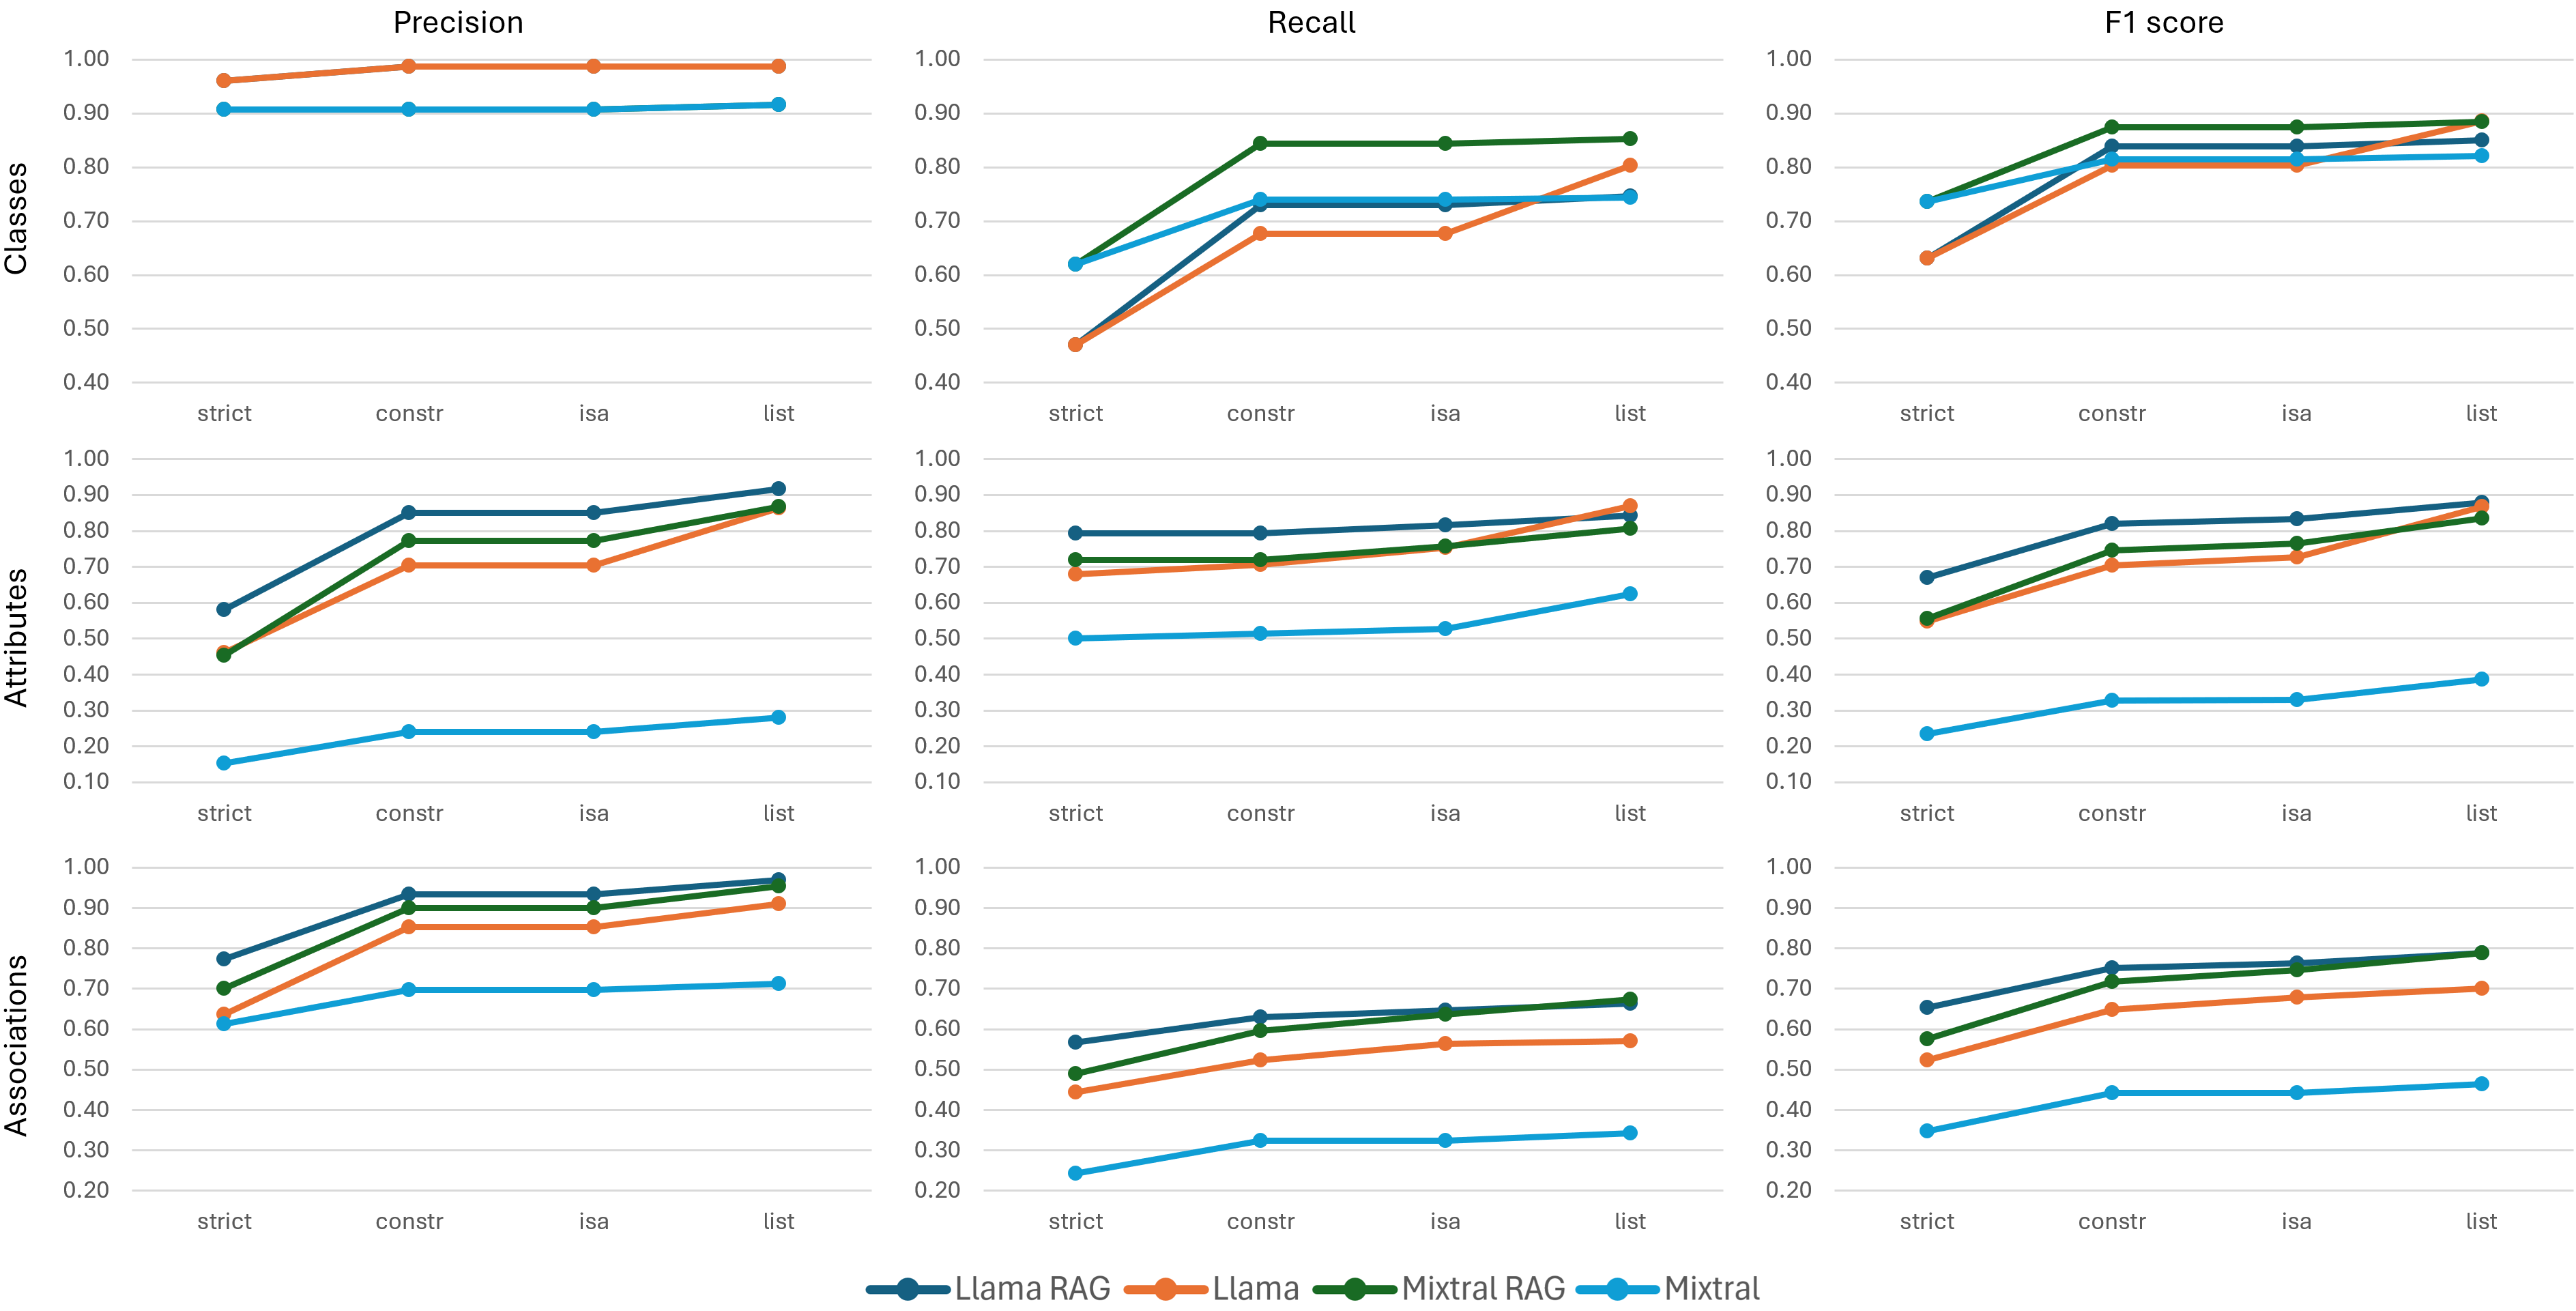
\includegraphics[scale=0.10]{img/evaluation-complex-p-r-f1.png}
    \caption{\centering Average Precision, recall and $F_1$ scores for the complex domain descriptions at the four levels of matching strictness}
    \label{fig:evaluation-complex-p-r-f1}
\end{figure}

\begin{figure}[!h]
    \centering
    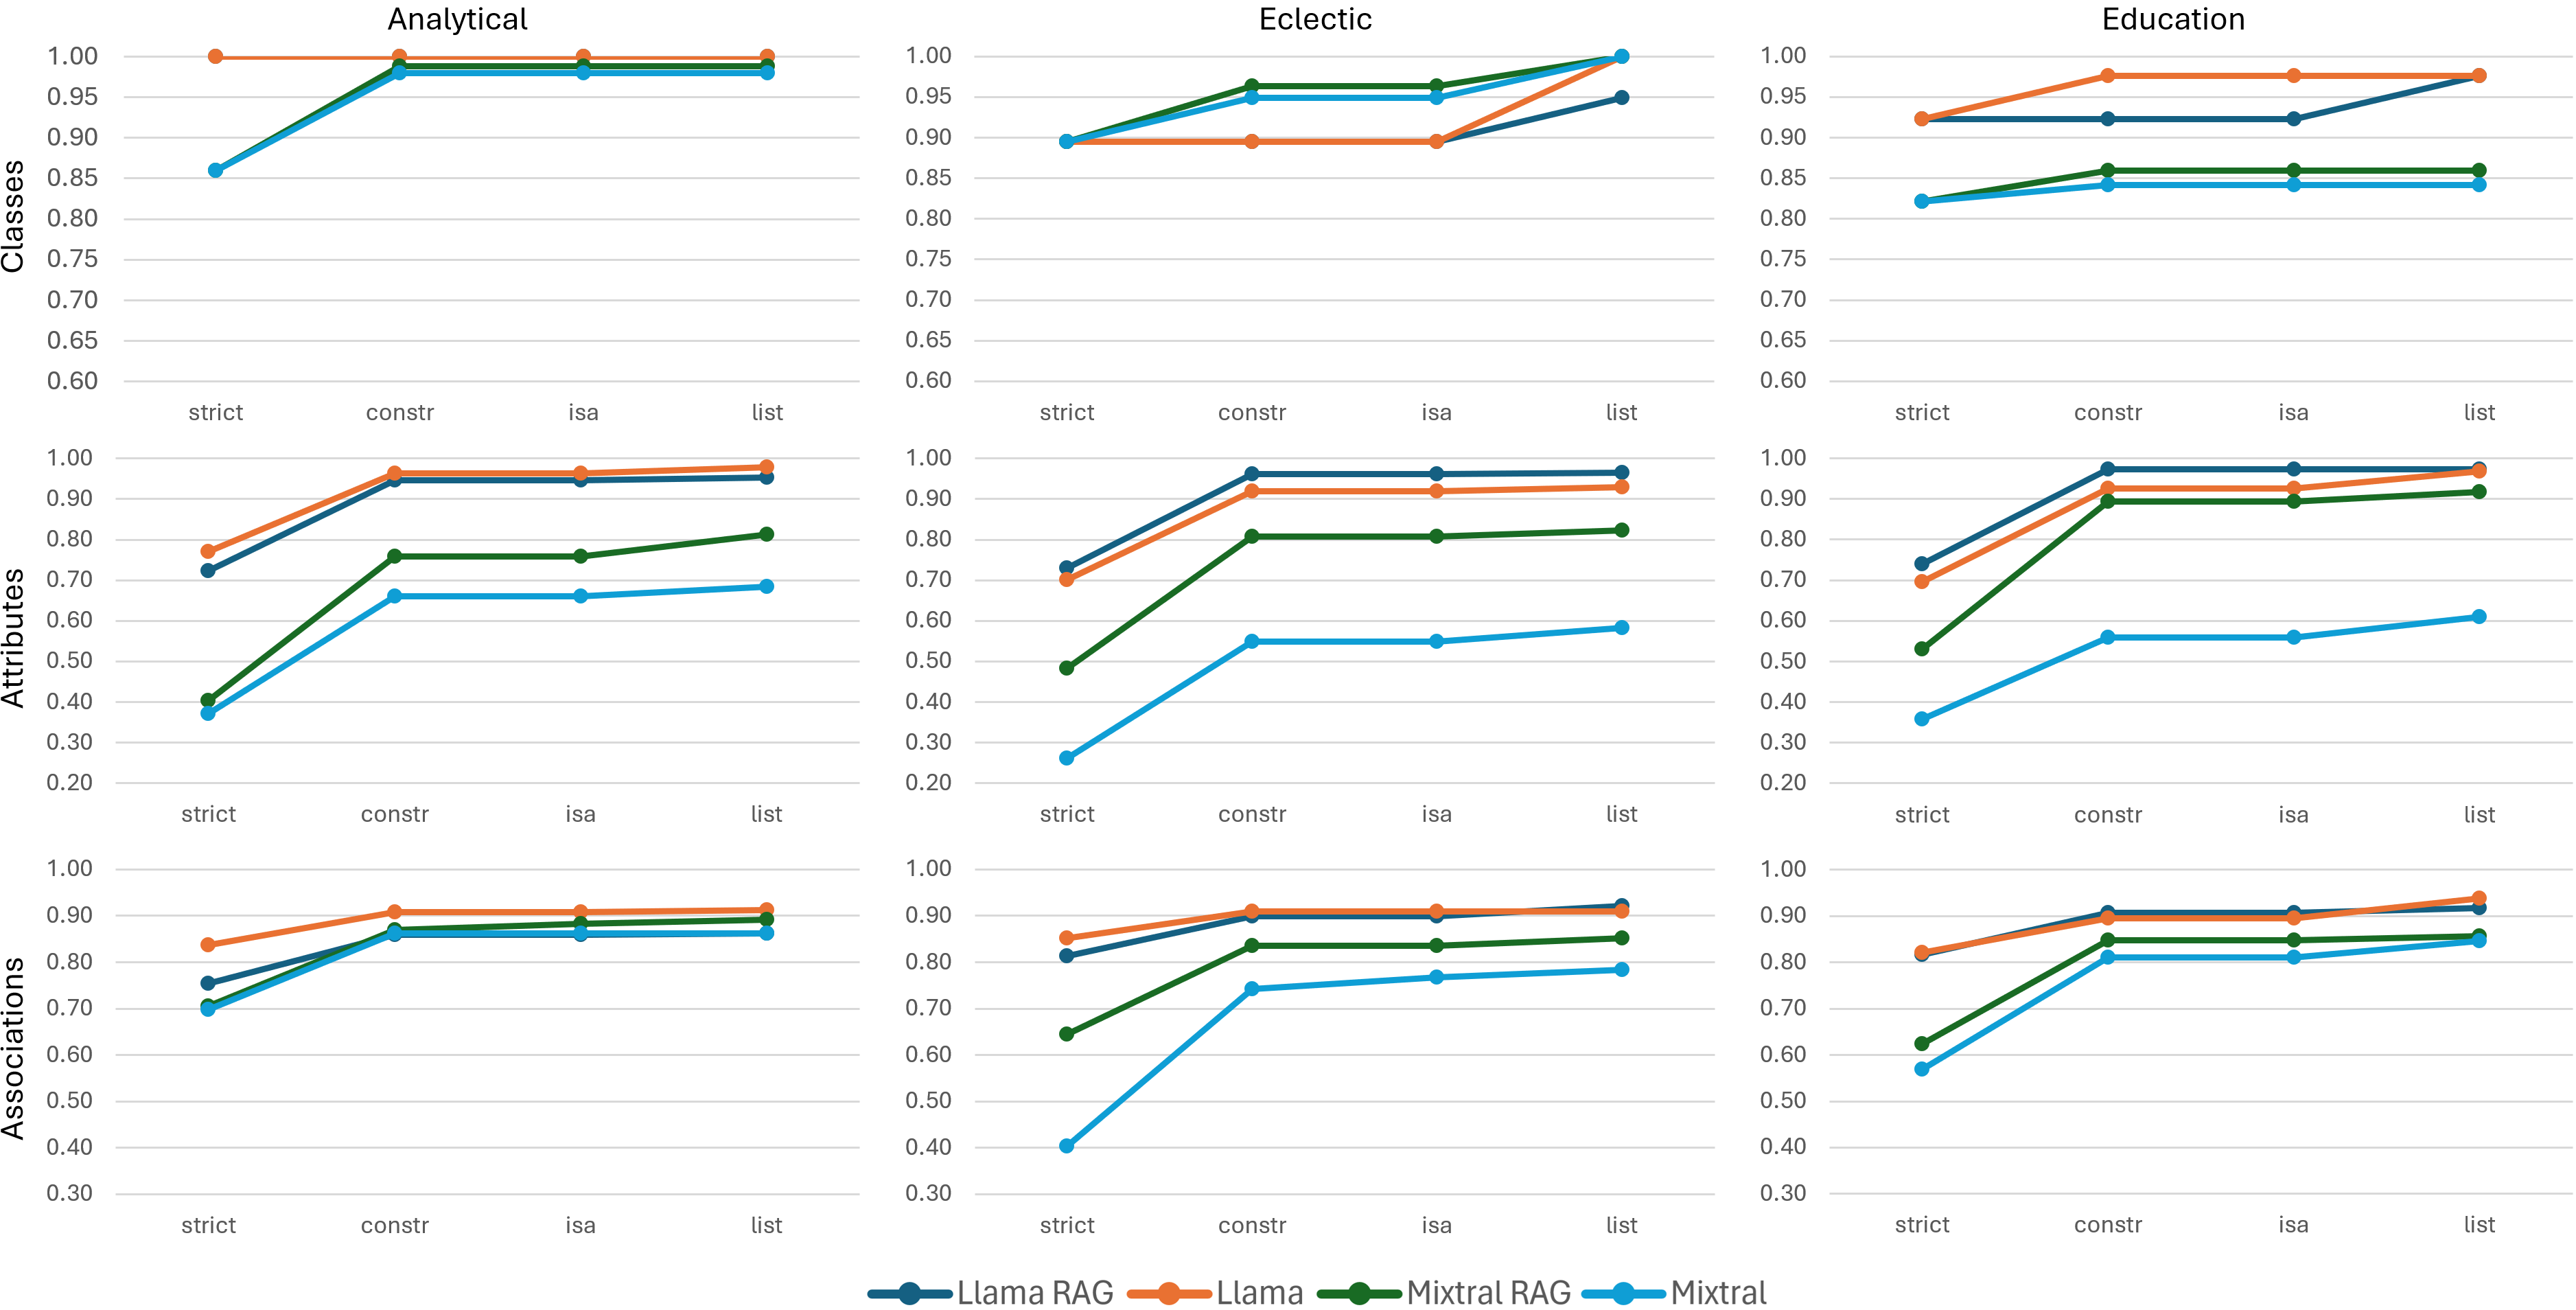
\includegraphics[scale=0.10]{img/evaluation-simple-f1.png}
    \caption{\centering Average $F_1$ score for the analytical, eclectic, and educational domain descriptions at the four levels of matching strictness}
    \label{fig:evaluation-simple-f1}
\end{figure}


\subsubsection{Overall performance}

The results indicate that Llama generally performs better than Mixtral.
This difference is clearly visible for the simpler evaluation domains in all description styles.
In contrast, for complex domains with intricate descriptions, the performance gap narrows.
Notably, Mixtral with RAG surpasses Llama without RAG in suggesting attributes and associations within complex domains.
Both models show the highest performance in suggesting classes.
They are comparable in suggesting attributes and associations, which is given by the duality in their manual evaluation.
The average precision for classes on complex domains is the same with and without RAG, as RAG is not used for classes.


\subsubsection{Impact of Introducing RAG}

Introducing RAG improves the performance of both models.
For Mixtral, RAG significantly improves the $F_1$ scores for attributes and associations across all domains, making its performance almost comparable to Llama without RAG and even slightly better for complex domains.
This suggests that RAG can compensate for the smaller size of the Mixtral model when identifying properties modeled as attributes or associations.
This finding is crucial for implementing the generators, since using a large LLM like Llama in the generators is very resource-consuming.
Even a simple RAG technique makes less demaning LLM comparable to the larger one for the implementation of the generators.
For Llama, the improvement with RAG is less pronounced but still noticeable, particularly for complex domains.
For classes, the impact of RAG is minimal, because the class generator always works with the entire domain description.
We can see some improvements in recall for the less strict levels of matching that also consider classes suggested as part of attribute and association suggestions, where RAG brings improvements.


\subsubsection{Domain and Style Specific Performance}

Both LLMs perform better in analytical and educational descriptions, probably due to the shorter, more structured, and consistent nature of these descriptions.
The eclectic and complex domain descriptions show more variability in performance.
Both benefit from introducing RAG which shows that diverse and less structured domain descriptions benefit from RAG even for large Llama.


\section{Descriptions evaluation}

We evaluated generated class descriptions based on the following questions:

\begin{enumerate}
\item [Q1:] Is the generated description solely based on the given domain description?
\item [Q2:] Is the generated description semantically corresponding to the given domain element?
\item [Q3:] Does the description not miss any useful information?
\end{enumerate}

To limit subjectivity of the evaluation, in the Q2 we consider the sets $S_1$ and $S_2$ that contain for the given class definitions of its attributes and its associations contained by the domain description and contained by the generated description. If the sets $S_1$ and $S_2$ have only a small intersection then we answer \textit{yes} to Q2, otherwise \textit{no}. For Q3 we consider the sets $T_1$ and $T_2$ of properties of the given class provided by the domain description and by the generated description. If the sets $T_1$ and $T_2$ have almost full intersection then we answer \textit{yes} to Q3, otherwise \textit{no}. For example, consider the following domain description: \\

\noindent{}\textit{A farmer is an individual engaged in agriculture identified uniquely by a name that is used to refer to the farmer from various documentation.} \\

\noindent{}and consider the following description for the class \textit{farmer}: \\

\noindent{}\textit{Farmer is an individual.} \\

\noindent{}Then in Q2, the set $S_1$ contains the definition of the name of the \textit{farmer} and the set $S_2$ is empty therefore, these sets have no intersection and the answer to Q2 is \textit{yes}. For the Q3 the set $T_1$ contains the information that the class \textit{farmer} is an individual, engaged in agriculture, and identified by a name. The set $T_2$ contains only that the \textit{farmer} is an individual therefore, the sets have only a small intersection and the answer to the Q3 is \textit{no}.

%\noindent{}TODO: Napsat, že jako popis domény jsme použili \emph{zoological gardens-00} \\

%\noindent{}TODO: Přidat výsledky měření a okomentovat je


\section{User-based evaluation of the application}

In addition to the measurements of the performance of the genererators, we also evaluated how real domain modelers accept an automated domain modeling assistant.

We prepared two domain descriptions, a summary of the main features of the prototype, and three 2-minute video tutorials.

We instructed real users to model the two domains and then asked them to assign a number between 0 (fully disagree) and 4 (fully agree) to express their agreement with five different claims about using our prototype tool.
They also classified themselves as teachers, students, modeling experts, database experts, programmers, or managers (multiple options were allowed).
We received responses from 18 users.

Figure \ref{fig:user-based-evaluation} shows for each type of users the number of responses that picked this type and the average marks received for that type. The last line shows the average of all users.

\begin{figure}[!h]
    %\centering
    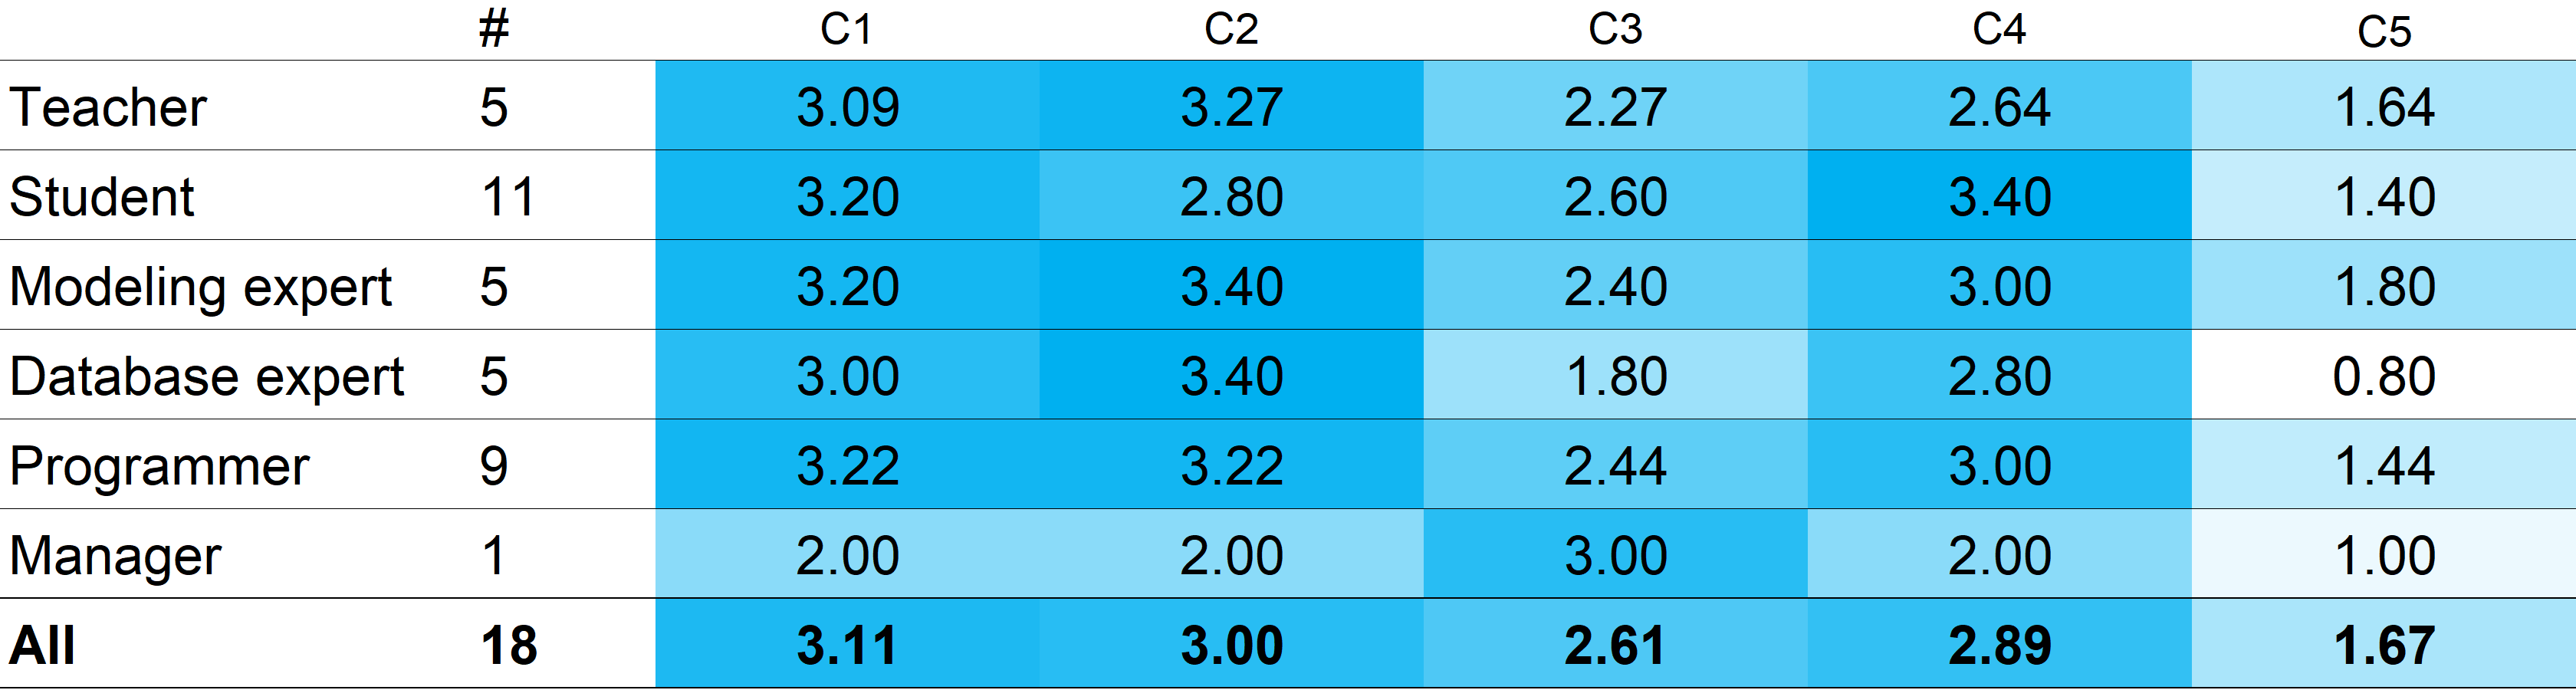
\includegraphics[width=1\linewidth]{img/user-based-evaluation.png} \\
    \scriptsize
\raggedright{C1: Modeling with the assistant is better compared to manual modeling. \\
C2: The assistant is intuitive to use.\\
C3: The assistant suggests appropriate classes, attributes, and associations.\\
C4: The assistant helped me solve the tasks faster compared to manual modeling.\\
C5: I solved all the tasks using only the assistant, and manual modeling was not needed.}
    \caption{Summary of the user-based evaluation. 0=fully disagree, 4=fully agree.}
    \label{fig:user-based-evaluation}
\end{figure}

As we can see, the users agree that using the automated assistant is better than pure manual modeling (C1) and found it intuitive (C2).
The suggestions provided by the tool are subjectively not always appropriate (Q3), which is also supported by our measurements presented in the previous part, and manual modeling is still necessary (Q5).
Despite these imperfections, users claimed that the prototype made them more productive (Q4).
We can find the weakest support in the manager category, but we were able to get only one response in this category, so a further evaluation is necessary.